\documentclass[border=10pt]{standalone}
\usepackage{tikz}
\usetikzlibrary{arrows.meta}

% ========== 配色 ==========
\definecolor{inFill}{RGB}{183,224,177}
\definecolor{inLine}{RGB}{32,102,32}
\definecolor{hidFill}{RGB}{199,203,243}
\definecolor{hidLine}{RGB}{52,58,143}
\definecolor{outFill}{RGB}{243,199,199}
\definecolor{outLine}{RGB}{143,52,52}
\definecolor{orFill}{RGB}{250,224,180}
\definecolor{orLine}{RGB}{190,110,20}
\colorlet{myblue}{blue!70!black}
\colorlet{head}{red!60!black}

\begin{document}
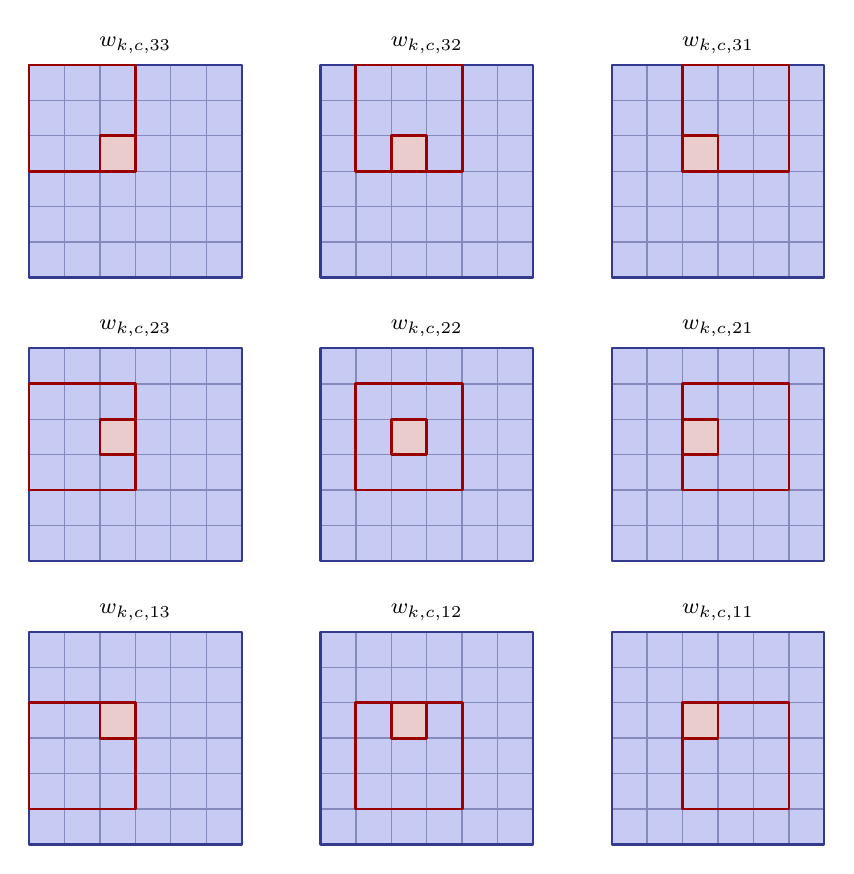
\begin{tikzpicture}[
    line join=round, font=\small, line width=.8pt,
    >={Latex[length=2.5mm, width=2mm]}
  ]

  % 单元尺寸
  \def\s{0.45}

  % ================= 3x3 排列的九张紫 6x6 =================
  \foreach \i/\j in {2/2,2/3,2/4, 3/2,3/3,3/4, 4/2,4/3,4/4} {
    \pgfmathsetmacro{\ox}{3.7*(\j-2)}      % ★ 宏名纯字母，不能再叫 \x0
    \pgfmathsetmacro{\oy}{14.4-3.6*\i}     % ★ 同上
    \pgfmathtruncatemacro{\wi}{5-\i}
    \pgfmathtruncatemacro{\wj}{5-\j}
    % ---- 紫 6x6 底 ----
    \fill[hidFill] (\ox,\oy) rectangle ++(2.7,2.7);
    \draw[step=.45, hidLine!60, line width=.5pt, shift={(\ox,\oy)}] (0,0) grid (2.7,2.7);
    \draw[hidLine, thick] (\ox,\oy) rectangle ++(2.7,2.7);
    % ---- (3,3) 位置填红 ----
    \fill[head!20] ({\ox+2*\s},{\oy+3*\s}) rectangle ++(\s,\s);
    \draw[head, line width=1pt] ({\ox+2*\s},{\oy+3*\s}) rectangle ++(\s,\s);
    % ---- 红 3x3 窗：输出 (i,j) 的卷积窗，必过 (3,3) ----
    \draw[head, line width=1pt]
          ({\ox+(\j-2)*\s},{\oy+(5-\i)*\s}) rectangle ++(3*\s,3*\s);
    % ---- 上：输出位置；下：对应权重 ----
    \node[font=\footnotesize] at ({\ox+1.35},{\oy+2.95}) {$w_{k,c,\wi\wj}$};
  }
\end{tikzpicture}
\end{document}